\section{Sprint 2}
This sprint was targeted towards getting some of the key features functional and in a state where the app could be used functionally. The initial proof of concept had some of the features like deck and card creation, user and organisation creation and the ability to view decks/cards linked to your organisation. The next major step was getting editing for all of the assets and tidying up the interfaces for managing the decks and cards.

\subsection{Improving Workflow of Cards and Decks}
One of the major problems identified with the work flow of the proof of concept was the disconnect between the list view and the creation of cards and decks. Initially creating a new card would bring up a separate screen with a separate url. This disconnects the content from the context of the deck or organisation. To improve the user experience when creating cards and decks, I implemented an inline feature for adding cards. To do this I changed the creation form to be displayed as a card the same as the current cards within the deck. This made it so when you start adding a card it will display it in the list and allow you to fill out the details within the card without changing changing page or view. 

 \begin{figure}
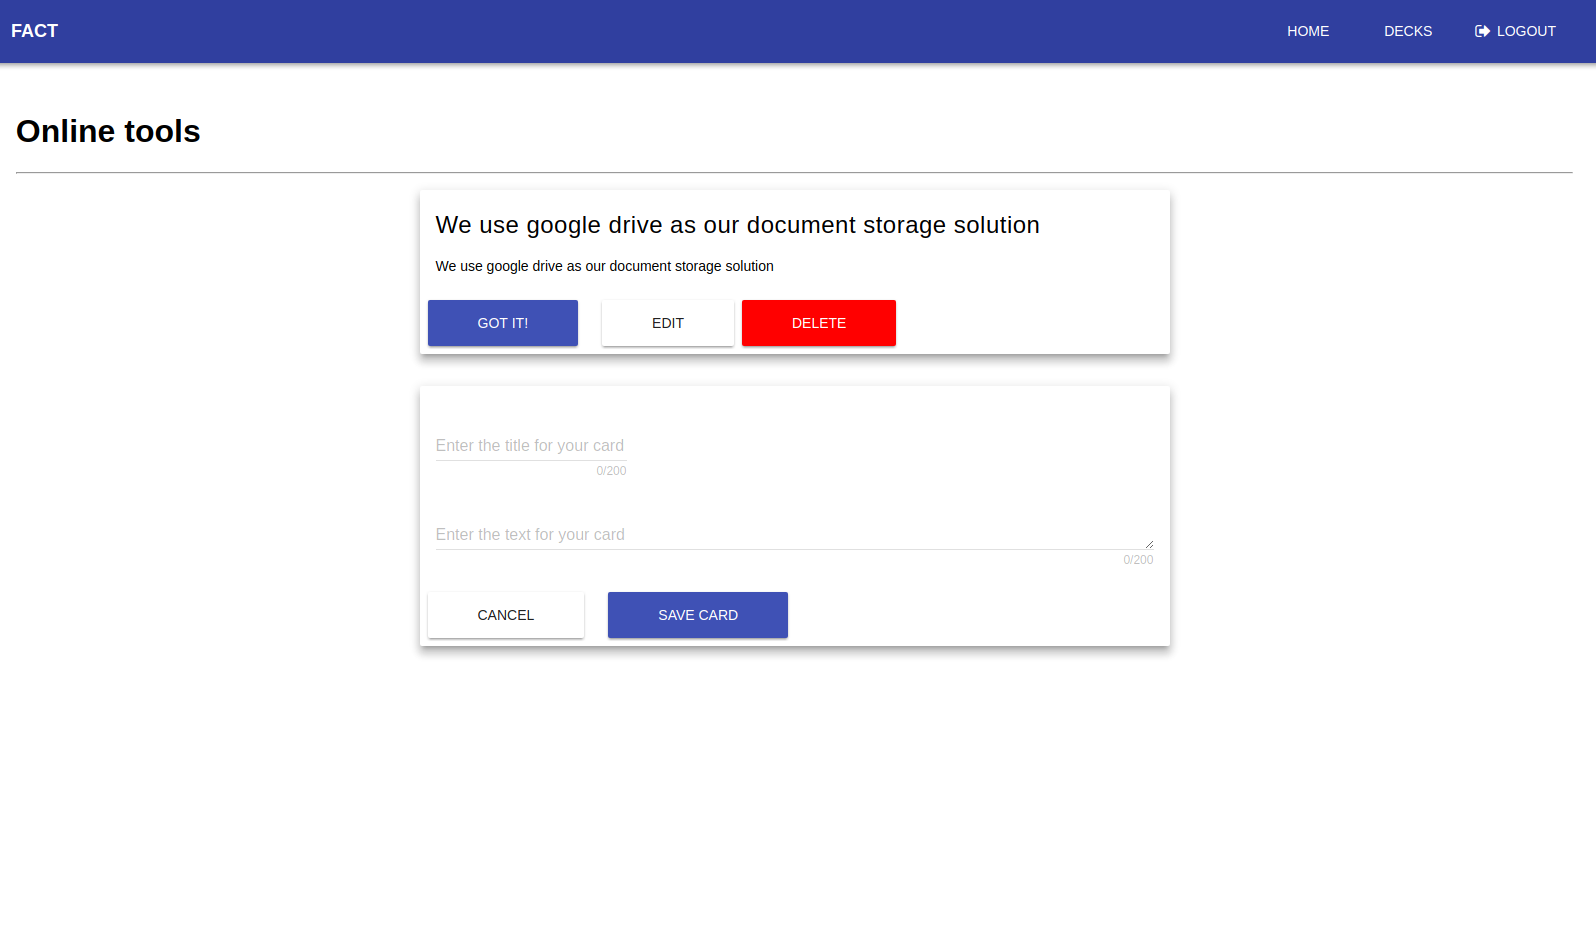
\includegraphics[width=\textwidth]{s2-edit-2}
\caption{Card creation after sprint 2}
\centering
\end{figure}


This change streamlined the user experience and made it more clear what the creation of cards and deck was doing and the general structure of the information. This in display creation and editing can be seen in many other web applications that use a card based display system such as Trello and Basecamp (see appendix: \ref{appendix:cardResearch}).

\subsection{Cards and Deck Editing}
During this sprint I added editing to the cards for both decks and cards this used the same system as the card creation just with different actions. This allowed me to reuse the same react component with different actions passed to it. This highlights the uses for react and the flexibility it brings when it comes to code reuse.

\subsection{Summary}
At the end of this sprint we went through the basic features that we needed to implement for a minimum viable product and identified some of the major ones that the product was still missing. It was also discussed about changing the component library we were currently using as it had limited design space and the overall default styling was not close enough to the final goal for the minimum viable product.